\documentclass{article}
\usepackage{graphicx}
\usepackage{hyperref}
\usepackage[a4paper, margin=1.25in]{geometry}
\usepackage{breakcites}
\usepackage{subcaption}
\usepackage{float}
\usepackage{textcomp}
\usepackage{amsmath}
\usepackage{textgreek}
\usepackage{authblk}
\usepackage{rotating}
\usepackage{booktabs}
\usepackage{longtable}
\usepackage{pdflscape}
\usepackage{lineno}
\usepackage{xcolor}
\usepackage[
  style=numeric,
  citestyle=numeric-comp,
  backend=biber,
  doi=true,
  natbib=true,
  sorting=none
]{biblatex}
\usepackage{scalerel,xparse}

\addbibresource{TextDataClimateShocks.bib}

% To be able to use emojis
\NewDocumentCommand\emojismile{}{
    \scalerel*{
        
\includegraphics{smiling-face-with-smiling-eyes_1f60a.png}
    }{X}
}

\begin{document}
%https://www.overleaf.com/project/5f918edd1afc380001feca0d
\title{Fine-scale Twitter Big Data Reveals Neighborhood Inequalities in Mental Health Effects of High Temperatures}

\author[1, *]{Matthew Cooper}
\author[2]{Jeremiah Osborne-Gowey}
\author[3]{Zheng Liu}
\author[4]{Jie Liu}
\author[5]{Portia Adade Williams}
\author[6]{Aaron Schwartz}
\author[7]{Patrick Baylis}

\affil[1]{T.H. Chan School of Public Health, Harvard University}
\affil[2]{University of Colorado Boulder}
\affil[3]{Department of Geographical Sciences, University of Maryland College Park}
\affil[4]{School of Business, East China University of Science and Technology}
\affil[5]{University of Cape Town}
\affil[6]{University of Colorado Boulder}
\affil[7]{University of British Columbia}
\affil[*]{Corresponding Author: mcooper@hsph.harvard.edu}

\maketitle

\begin{abstract}
%Limit 150 words: https://www.nature.com/nclimate/about/content
%Actually there are lots of examples of articles with > 150 words, but I think we should keep it concise
Higher temperatures associated with climate change are expected to have major impacts on human mental health.  Indeed, traditional analyses of heat and mental health outcomes using data collected by public agencies have found associations between elevated temperatures and increases in outcomes such as suicides and mental-health related hospitalizations.  However, these studies, which typically use data reported at the city or county level, have found no difference in vulnerability based on income.  We overturn this finding and show that there are stark differences in vulnerability using a novel data source: expressed sentiment in 250 million geolocated tweets, matched with prevailing weather as well as neighborhood economic and demographic conditions.  We find that increased temperatures worsen expressed sentiment in all areas, but that this effects is much stronger in poor and black neighborhoods.

\end{abstract}

Keywords: Text Data, Environmental Shocks, Social Media Mining, Sentiment Analysis, Topic Modeling, Social Media, Public Opinion, Perception, Sentiment, Media, News, Twitter, Climate Change, Science Communication, Policy, Planning, Methods, Text Mining, Natural Language Processing, NLP, Latent Dirichlet Allocation, LDA, Political Ecology, Politics, Resilience, Adaptation, Suicide, Mortality, Morbidity, Self-harm, 

    
%Cite this new paper: https://doi.org/10.1016/S2542-5196(20)30251-5
% And: https://eos.org/articles/long-term-drought-harms-mental-health-in-rural-communities and this is the conf. paper citation https://agu.confex.com/agu/fm20/meetingapp.cgi/Paper/771750
\section{Introduction}

% Organize as follows:

% Heatwaves are known to worsen mental health
% AND mental health is strongly associated with income
% AND wealthier better able to cope with heatwaves 
% BUT we know little about the interaction between heatwaves, mental health and income
% THEREFORE: we did this really novel study.

% Jeremiah Osborne-Gowey: Randy Olsen (of "Don't be such a scientist" fame) and his ABT - And But Therefor framework for communicating - https://www.huffpost.com/entry/and-but-therefore-randy-o_b_8813330
% Jeremiah Osborne-Gowey: https://blogs.scientificamerican.com/observations/how-the-word-but-could-save-the-world/


This work builds on existing work by \citep{baylis_weather_2018}. 




%Intro Paragraph
% I think this should be more about climate change and mental health broadly, as well as a bit about how income has been theorized to affect vulnerability, but there is no evidence yet.  This can be shorter as well, as we have a lot of detail in the Background section 
% Cite this high-level study: https://www.nature.com/articles/s41558-018-0102-4/
% Also this review article saying more research is needed https://www.sciencedirect.com/science/article/pii/S0033350618302130
% -Matt

Research has shown strong linkages between ambient environmental conditions and mental health, with extreme temperatures  frequently associated with poorer overall mental health. Individual's mental health is strongly associated with income with people in lower income levels frequently experiencing higher stress levels and less able to find help for coping with these stresses. Other research on how people cope with environmental temperature extremes indicate that wealthier are better able to cope with heatwaves, whether from traveling to cooler climes, accessing air conditioning, or other temperature ameliorating strategies that may require access to financial capital. Yet we know relatively little about the interaction between temperature, mental health and income. Furthermore, previous studies that did attempt to examine relationships between environmental extremes and health sometimes aggregated data at scales too coarse to examine whether income may be an ameliorating factor. This study examines the interactions between these three using relatively fine-scale, publicly available data. Our research expands on existing studies of temperature and sentiment - one measure of mental health - by examining finer-scale data and incorporating income data to examine correlations between temperature extremes and sentiment.

Human moods and mental states are important aspects of overall well-being and can be influenced by ambient, persistent and fluctuating environmental conditions. Climate change is accelerating the rate and variability around meteorological norms like the timing, magnitude, intensity and duration of precipitation events and air temperature minima and maxima \href{https://www.ipcc.ch/site/assets/uploads/2018/03/SREX-Chap3_FINAL-1.pdf}{(link)}. Previous work \citep{baylis_weather_2018} indicate important linkages between human mood and meterological conditions. Previous analyses of the effects of weather on mood (as expressed in sentiment of text-based message), however, were constructed at the aggregated city/day level and did not account for differences in socio-economic status which may affect access to resources (e.g., air conditioning) that can offset the effects of exposure to temperature extremes. Here, we build on these previous studies by examining the hourly effects of weather on human sentiment, an expression of mood, exploring geographic and economic heterogeneity at a finer-scale resolution than previous studies.  

% https://medinform.jmir.org/2020/1/e16023/?utm_source=TrendMD&utm_medium=cpc&utm_campaign=JMIR_TrendMD_0
\section{Background}
\subsection{Temperature and Mental Health}
%Jeremiah Osborne-Gowey: We report on physiological and mental health in text here. Maybe just a heading of "health"?
%I think physical health is beyond the scope of this paper -Matt

%https://www.pnas.org/content/115/43/10953
Higher temperatures are associated with many indicators of worsened mental health.  Multiple studies have found strong evidence that higher temperatures are associated with increases in suicides in the United States \citep{Burke2018Aug, Mullins2019Dec, Dixon2007May}, and many others have demonstrated the same relationship around the world \citep{Qi2014Dec, Page2007Aug, Likhvar2011Jan}.  In addition to suicide, other research has found effects temperature on hospitalization events related to mental health disorders such as bipolar disorder and schizophrenia \citep{Mullins2019Dec, Lee2007Jan, Shapira2004Feb, Sung2013Feb, Gupta1992Jun, Hansen2008Oct}.

Temperature has been hypothesized to impact mental health through a number of pathways.  Work on biological mechanisms emphasize that there may be mental health effects from maintaining stable body temperature in high heat \cite{Lohmus2018Jul}.  Additionally, recent studies have found that nighttime temperatures affects sleep quality \citep{Obradovich2017May, Mullins2019Dec}

% The pathways
Higher temperature associated with climate change could influence mental health directly by exposing people to trauma. It could also indirectly influence mental health by affecting (1) physical health and (2)community wellbeing\citep{RN1314}. For the direct influence pathway, extreme heat events or increasing temperatures have been associated with the increase in aggression,higher suicide rates and other hospital admissions(Anderson and Anderson 1998,Cheatwood 1995; Cohn et al. 2004,Bouchama et al.2007.). Heat exposures in working environments could also reduce people's capacity to deal with physical and mental task, and increase the risk of accidents, because of the excessive core body temperature and dehydration((Bridger 2003; Kerslake 1972; Kjellstrom et al.2009d,Leithead and Lind 1964,Schrier et al. 1970). The loss of work capacity would in turn result in loss of income, which could also cause mental health problems(Kjellstrom 2009b).%% more physiological terms 

As for the indirect pathway, first, because of the reciprocal causation relationship between physical health problems and mental health problems(Miller et al. 2009; Prince et al. 2007), heat exposures associated with climate change along with other climate events and indirect health risks threatening physical health will directly influence mental health((Berry 2007,World Health Organization 2008b). Second,disordered temperature associated with climate change may destroy the economic in agricultural-production-dependent communities. For example, extreme heat reduces the work capacity of laborers in farm fields(Kjellstrom et al. 2009d), which further destroys agricultural-supported industries in local area(Berry et al. 2008). The following economic pressures would undermine social capital and then lead to mental health problems.

% Heatwaves are known to worsen mental health



https://doi.org/10.1016/j.puhe.2018.06.008 (review study - will have more to cite)
https://www.nature.com/articles/s41558-018-0222-x
https://ehp.niehs.nih.gov/doi/full/10.1289/ehp.11339
https://ijmhs.biomedcentral.com/articles/10.1186/s13033-018-0210-6
https://www.nature.com/articles/s41558-018-0102-4/
https://doi.org/10.1016/j.jhealeco.2019.102240

[ADD SUICIDE DATA TO HEALTH SECTION?]
https://www.psychologytoday.com/us/blog/greening-the-media/201809/global-warming-and-suicide

\subsection{Mental Health and Vulnerability}
% This is good, but probably should be shortened.  Maybe one para showing that income matters, one para discussing pathways, also maybe focus/change phrasing to be more on "vulnerability" -Matt

% AND mental health is strongly associated with income
% 1)Childhood 2)adulthood 3)gender
% Perceived income level

% Talk more about race
% This is interesting: https://www.pnas.org/content/118/17/e2019624118.abstract?etoc

The relationship between income, socioeconomic status (SES), well-being and mental health is one of the strongest established patterns in psycho-social literature \citep{Easterlin1974Jan, holzer1986increased, Perry1996Sep} (I cant find Ng et al. 2014). Much of the research into these patterns focuses on the inequalities and distribution of the effects on individual well-being. Subsequent work on mental health outcomes, one measure of well-being, have established strong associations between SES, income and mental health with the most and least privileged most commonly associated with the best and worse mental health experiences and outcomes, respectively \citep{Sevenson2008Aug}(cites: Ng et al. 2014). 

For example, results from a cross-sectional comparative study of socioeconomic factors and use of mental health services by people living in Ontario, Canada and the United States, indicate clear disparities in use of mental health services between those with the highest income levels and lowest mental health morbidity and those with the lowest income levels and highest mental health morbidity - those with higher incomes tended to have lower mental health morbidity issues while utilizing mental health services more than those with lower incomes and higher mental health issues \citep{Katz1997}. 

Results from a systematic review of the literature on associations between social inequalities and mental health disorders indicate a clear and prevailing link between  one or more indicators of less social privilege and higher prevalence of mental health disorders \citep{Fryers2003}, with low income one of the most consistent markers of and associations with increases in common mental health disorders. Collectively, results from the income and mental health literature indicate that socially disadvantaged populations experience significantly more frequent common mental health disorders. Scholars use mental health disparities to indicate the disproportionate amount of mental health disorders among persons of low SES \citep{RN1292}

The established association between poverty and mental health revealed that that income distribution may have a significant influence upon mental health over and above the effect of poverty \citep{HANANDITA201459}.Poverty has been identified as one of the major risk factors in mental health. For instance, some systematic reviews have shown that socioeconomically disadvantaged children and adolescents were 2-3 times more likely to have mental health problems than others\citep{REISS201324}, while the household increases in financial resources are generally associated with an overall reduction of mental health problems\citep{2015Does}. Others have argued that increases in SES can serve as a buffer against the negative impacts of difficult life experiences on mental health, particularly for individuals already under substantive mental stress \citep{Kawachi2001Sep}. Thus, SES and income are associated with mental health improvements in SES and income can serve to decrease mental health problems.

 
Several reasons could explain why poverty may effect mental health. 1) the “social causation hypothesis” which suggests that stress or deprivation or decreasing the likelihood of people getting treatment may lead to poor mental health\citep{mills2015}, while social capital could reduce the likelihood of living in poverty and reduces the risk of mental disorders such as depressive symptoms and suicidal tendencies\citep{RN1291}. 2) negative life events in a person’s life such as job loss are also associated with the risks of poverty\citep{RN1293} and mental health\citep{TAMPUBOLON201420}, and the causal inferences on the effect of poverty and mental health had also been made in several studies. For example, Tampubolon and Hanandita\citep{TAMPUBOLON201420} find that individual social capital is positively associated with mental health while adverse events were negatively associated; Chang.et.al \citep{RN1291} find that subjective and objective poverty is significantly associated with a higher risk of adverse life events, less social support and mental distress. Negative life events and social support in serial mediate the relationship between subjective poverty and mental health.

% jieliu.cnah: Could delete
For children, poverty and poor maternal mental health often co-exist and are two of the risk factors for child development\citep{LUND20111502}, and maternal mental health is significantly associated with child general psychopathology\citep{ RN1289}. Researchers also find that transition into poverty increased children’s socioemotional behavior problems and maternal psychological distress \citep{WICKHAM2017e141}.

In general, the relationship between mental health and income level is well established. In the study, we explore whether income level would influence the link between weather and the sentiment in Twitter-posed text.

https://jamanetwork.com/journals/jamapsychiatry/fullarticle/211213
https://doi.org/10.1002/9781118410868.wbehibs570
https://www.sciencedirect.com/science/article/abs/pii/S027795362030527X
https://www.sciencedirect.com/science/article/pii/S2468266717300117
https://doi.org/10.1016/S2468-2667(17)30011-7
https://link.springer.com/article/10.1007/s00127-017-1370-4
 % Jeremiah Osborne-Gowey: Not as relevant. Saved the citation but didn't find enough relevant text to include reference to here in our manuscript. Maybe this: https://journals.plos.org/plosone/article?id=10.1371/journal.pone.0116820
https://www.sciencedirect.com/science/article/abs/pii/S0143622814002537
also this: https://www.sciencedirect.com/science/article/abs/pii/S0140673614614604

\subsection{Income and Temperature}
% AND wealthier better able to cope with heatwaves 
https://www.nature.com/articles/nclimate3253
https://www.sciencedirect.com/science/article/abs/pii/S0378778818321327
https://www.mdpi.com/2225-1154/8/1/12/htm

NOT CLEAR: https://doi.org/10.1016/j.jhealeco.2019.102240 and https://www.nature.com/articles/s41558-018-0222-x find little evidence of adaptation

% BUT we know little about the interaction between heatwaves, mental health and income


% THEREFORE: we did this really novel study.
https://www.nature.com/articles/s41598-017-12961-9

%OTHER LEFTOVER TEXT TO MAYBE BRING IN LATER



Meteorological conditions can impact human physical (cite) and emotional states (cite). Emotional states and well-being are associated with physiological functioning and mental acuity which can affect social relationships, workplace productivity (cite) and health risks (cite). People that are more reliant on 1) livelihoods which require them to be outdoors (e.g., farming, agriculture, logging, etc.), 2) living and working in places where they are exposed to environmental minima and maxima, or 3) with prolonged exposure to ambient meteorological extremes are particularly vulnerable to changes in environmental exposure \citep{frimpong_heat_2017} and associated health risks (cite). Exposure to extreme environmental conditions can also have implications for workplace productivity and livelihoods \cite{kjellstrom_impact_2016}. For example, Nigerian maize farmers experience significant declines in productivity (2-8percent per degree above 17degC) along with substantive increases in health impacts including dehydration, muscle cramps, headaches and dizziness, heat exhaustion, sun stroke, and even death \cite{sadiq_impact_2019}. Other research indicates farm health and labor productivity were compromised under extreme heat and cold events in the Nepali Food Bowl region \cite{budhathoki_socio-economic_2019}. Similarly, Oregon farmers reported health impacts of working in both hot and cold conditions but the negative impacts were attenuated relative to the high heat situations \cite{bethel_heat-related_2014}. Other research found occupational injuries in Thailand increased with increasing heat exposure and occupational heat stress \cite{tawatsupa_association_2013}. Heat exposure risks are also a key factor in urban areas with particular attention needed for how the impacts of changing climate play out in health inequality \cite{friel_urban_2011}. 

Current estimates place annual workplace productivity losses due to heat exposure at 15-20percent with that rate potentially doubling by 2050 \cite{kjellstrom_heat_2016}. Projected increases in future ambient temperature suggest serious short- and long-term potential health consequences from exposure to heat stress (cite) with some estimates putting potential productivity losses at several percentage points by 2030 \cite{kjellstrom_heat_2016}, with middle- and low-income countries particularly vulnerable as they are often more reliant on physical work for their livelihoods. 

The level of changes in weather influences people’s mental health and patterns of emotions expressed. A study by Sun et al. 2018 \href{file:///Users/portia/Downloads/ijerph-16-00086-v2 20(1).pdf.}{(Portia has this PDF?)} demonstrates varied relationships between haze and negative emotions of the public under different seasons of the year. Being sad or happy influences one's style and value of reasoning. Time of day, season, location, and climate allow aggregate prediction of sentiments \cite{hannak_tweetin_2012} \href{https://www.ccs.neu.edu/~amislove/publications/Weather-ICWSM.pdf}{(link to PDF)} while positive affect from an evaluative statement enhances potential responses \cite{clore_how_2007} \href{https://www.ncbi.nlm.nih.gov/pmc/articles/PMC2483304/pdf/nihms40349.pdf}{(link to PDF)}. For instance, changes in temperature affects people’s response about weather. Depending on a reference temperature for an  area and time of year, people are more likely to comment on unusual weather for a particular place and time than on the same weather considered typical in another place \cite{moore_rapidly_2019}.

% Jeremiah Osborne-Gowey: Remove parts of this paragraph that relate to call for international research on these linkages as we now are only focusing on USA for Tweets.
Although climate change is an international phenomenon experienced in every country, its discussions vary from country to country. According to Vu and others \cite{vu_nationalizing_2019}, a country’s climate severity, economic status and governance determine variations in its media discussions. 
% Jeremiah Osborne-Gowey: I think we can remove this entire paragraph now as it's outside the focus of this paper. Might be relevant for our 2nd paper!
When removing the paragraph, cut from here and copy to the end of the doc where we have extra text saved. [DO NOT DELETE, just move from here]

% Jeremiah Osborne-Gowey: This is perhaps the only piece of this paragraph still relevant for this paper...
For example, Park and others \cite{park_mood_2013} \href{https://pdfs.semanticscholar.org/b282/feb759e57530b115dcc4bb080f96598a5246.pdf}{(link)} demonstrated that many people living in a state with higher mean temperature express more positive emotions on Twitter than those living in colder states in the US. Schmidt and others \cite{schmidt_media_2013} posit that climate severity and environmental factors related to carbon dependency influences the amount of coverage climate change receives in the media in countries like USA, Australia and Germany. Studies comparing how different countries portray climate change have been widely conducted in USA, UK, France and the Netherlands \cite{vu_nationalizing_2019}. Such comparisons are mainly between developed countries with developing countries outside the focus.  Schafer and O’Neil \cite{schafer_what_2013} advance the need for academic scholars to investigate transnational contexts within climate communication. Wealthier countries with comparatively higher GDP are likely to frame climate change as a political issue as financial resources exist for exploring research on climate change. Conversely, coverage of climate change news from poorer developing countries focus mainly on international relations. Thus, the effects of national macro economic variables that affects a country’s sociopolitical and economic development such as GDP reflects a country’s governance system in media coverage \cite{vu_what_2018}. Cultural theorists assert that, understanding such differential variations depicts how different entities interpret danger and respond to risk \cite{tansey_cultural_1999}. Inclusion of developing countries in scientific research provides an avenue for international support to such countries in responding to the effects of climate change.Yet studies attempting to explain cross-national variation in climate change public opinion is limited \cite{knight_public_2016}.

Public debates on the current consequences of climate change are discussed in both scientific and non-scientific mediums. 
% Jeremiah Osborne-Gowey: Need a better transition here between meteorological conditions and effect on mood (expressed as sentiment). Feels like we're missing a discussion (new paragraph?) just above here that discusses this. This might be where we plug in the text PAW is working on?
People can express their emotional states and feelings - sentiment - through physical, vocal and written expressions on mediums including newspapers, scientific articles, blogs and other online social media platforms. Twitter is one of the more popular social media platforms where people express their sentiments about any number of topics. Public posts on Twitter - called tweets - are widely available for public consumption and research, and offer a glimpse into collective social state. For example, text posted to these platforms can be used to gauge the public mood, assess opinions, measure brand affinity and for emergency planning and disaster response (cites). 
% Jeremiah Osborne-Gowey: Good to cite the top-cited public opinion papers, the Twitter flood study from CU, others from data science field including another Baylis paper
Sentiment is frequently employed as a correlate of emotional state or mood (cites). Weather events focus public attention in different ways of expression (cites). These data offer a unique opportunity to analyze how people express and respond to events in people's daily lives, including their exposure to ambient environmental conditions.



Here, we report on associations between meteorological conditions and expressed sentiment of public posts on Twitter from the United States of America (USA) between 2009 and 2019. This work builds on research from Baylis and others \cite{baylis_weather_2018} on weather impacts on expressed sentiment. In particular, we extend this work by including the temperature effects on sentiment in multiple regions across the USA while drawing in various climatic variables and socio-demographic data. In this research, we explore two primary questions. First, to what extent are amibent environmental conditions correlated with changes in expressed sentiment? Second, is this effect moderated by wealth? and local land cover conditions?

Building on previous findings from Baylis and others, we hypothesize that local ambient environmental conditions have a strong connection how people are feeling as expressed in the sentiment of text messages posted on Twitter [H1]. Second, we hypothesize that the weather-sentiment link will be stronger in low-income areas. That is to say, people in lower income areas will be have lower sentiment scores than those in wealthier areas. [H2].

\section{Results}

\subsection{Overall Effect}
We examined the relationship between the sentiment expressed in tweets and the prevailing Wet Bulb Globe Temperature (WBGT), an indicator of heat stress that accounts for temperature, humidity, wind speed, and solar radiation.  Controlling for a variety of fixed effects, we found that, across all tweets, higher temperatures are associated with lower sentiment (See Fig. \ref{fig:wbgt}).  Sentiment is highest at a WBGT of 5\textdegree Celsius (a dry bulb temperature typically around 12\textdegree C/54\textdegree F).  The greatest declines in sentiment are observed between 20\textdegree -25\textdegree C WBGT (dry bulb 29\textdegree-36\textdegree C/84\textdegree-97\textdegree F).  Sentiment also declines with colder temperatures, but only slightly.  We ran models using multiple sentiment indicators, and found similar results no matter which sentiment metric was used (See Appendix).

\begin{figure}[H]
  \centering
  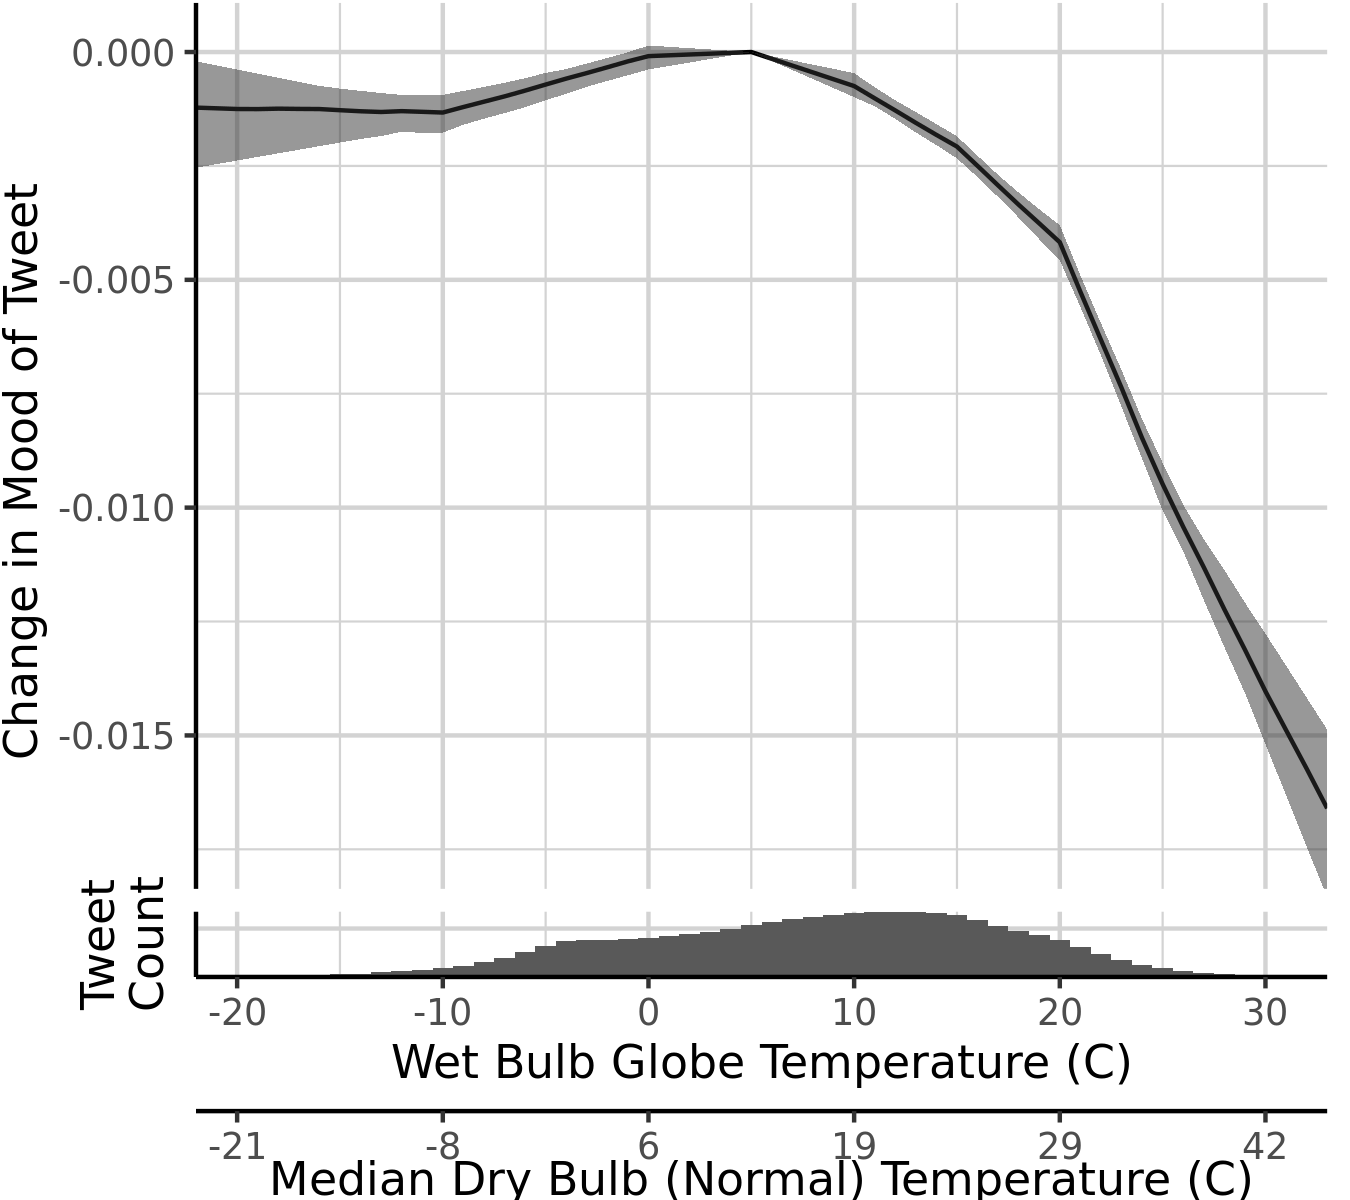
\includegraphics[width=0.5\linewidth]{../res/wbgt.png}
  \caption{Relationship between Wet Bulb Globe Temperature (WBGT) and sentiment in tweets.  As temperatures increase, sentiment declines.}
  \label{fig:wbgt}
\end{figure}

We then explored how the racial and income characteristics of neighborhoods moderate the relationship between WBGT and sentiment (See Fig \ref{fig:sub1}).  We found that neighborhood income strongly moderates the relationship between temperature and sentiment.  As temperatures increase to moderate heat of 20\textdegree C WBGT (29\textdegree C/84\textdegree F), sentiment decreases for most neighborhoods, but increases in neighborhoods in the 95th income percentile.  These rich do not see decreases in sentiment until temperatures are above 20\textdegree C WBGT (29\textdegree C/84\textdegree F), at which point sentiment decreases evenly across income ranges, still leaving a large gap in expressed sentiment from low to high-income neighborhoods.

We examined patterns of temperature and sentiment for neighborhoods that had a majority population of four broad racial categories - non-hispanic black, non-hispanic white, hispanic of any race, and other, which includes native american, multi-racial, and asian-american and pacific islander.  While people in neighborhoods of all racial compositions were affected by heat, people in majority black neighborhoods were much more affected than others  (See Fig \ref{fig:sub2}).  Relative to an optimum temperature of 5\textdegree C WBGT (12\textdegree C/54\textdegree F), as temperatures increase to 30\textdegree C WBGT (42\textdegree C/108\textdegree F), the sentiment of tweets in majority black neighborhoods decreases four-times as much as people in other neighborhoods.  Additionally, at levels of moderate heat from 10\textdegree C WBGT (19\textdegree C/66\textdegree F) to 25\textdegree C WBGT (36\textdegree C/97\textdegree F), people in majority hispanic neighborhoods have slightly lower sentiment than people in majority white or other neighborhoods, although this gap closes with high temperatures.

Finally, we modeled the combined effects of race and income in moderating the impacts of heat on mental health, and we found separate effects for these two variables (See Appendix).  In other words, neither race or income alone account for all the heterogeneity in vulnerability, and neighborhoods that are poor and black are more affected by than than neighborhoods that are just poor or just black.

\begin{figure}[H]
\centering
\begin{subfigure}{.5\textwidth}
  \centering
  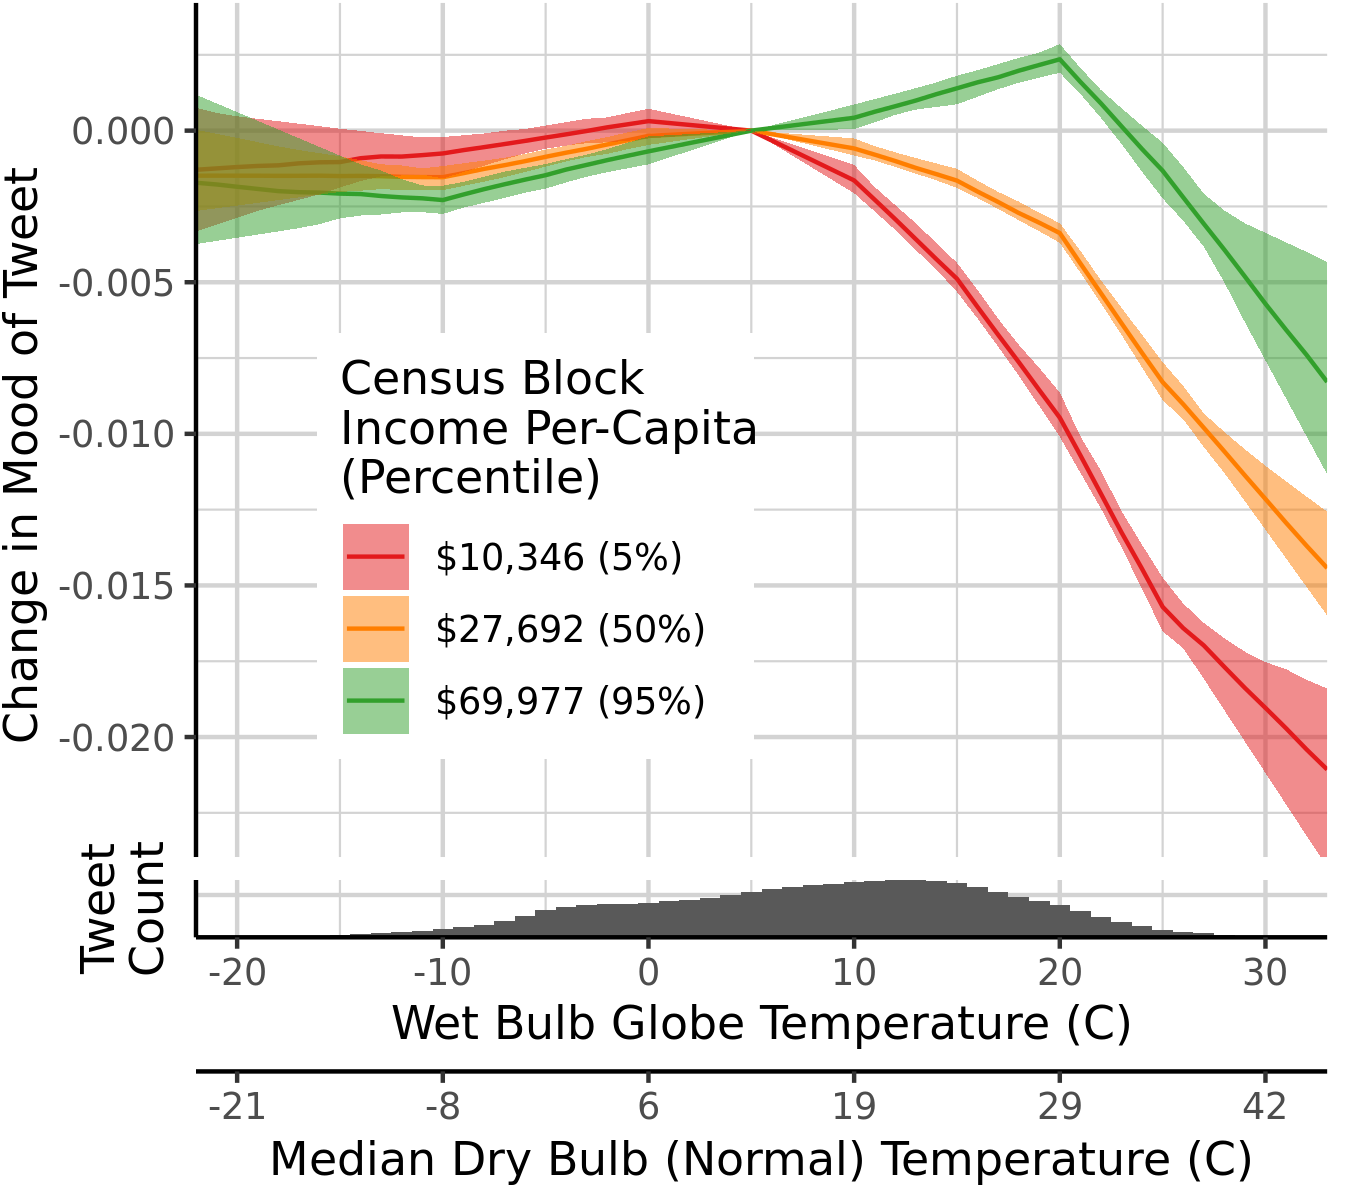
\includegraphics[width=\linewidth]{../res/wbgt-income.png}
  \caption{}
  \label{fig:sub1}
\end{subfigure}%
\begin{subfigure}{.5\textwidth}
  \centering
  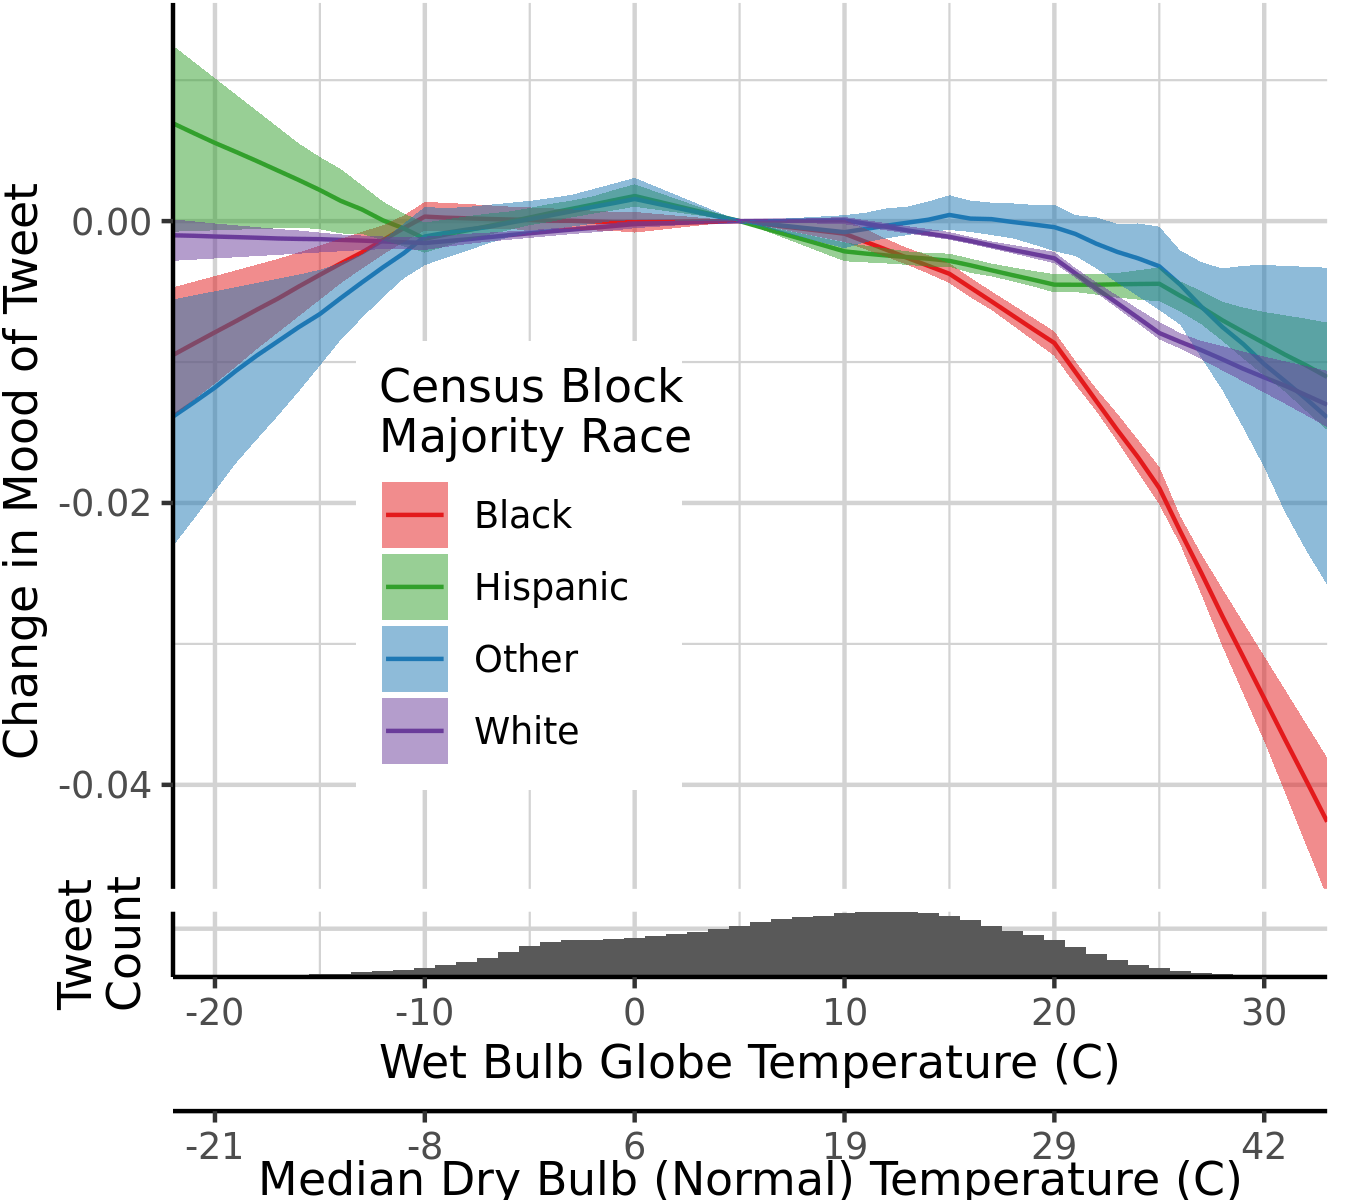
\includegraphics[width=\linewidth]{../res/wbgt-race_q.png}
  \caption{}
  \label{fig:sub2}
\end{subfigure}
\caption{Effect of changes in wet-bulb globe temperature on expressed sentiment relationship as moderated by neighborhood income (a) and race (b).}
\label{fig:test}
\end{figure}


\subsection{Comparison With Other Events}

Expressed sentiment is a widely used metric to assess mental health and well-being on social media.  While, a variety of related metrics can be used to quantify sentiment, we chose to use the VADER metric that was specifically designed for microblogs like twitter \cite{hutto2014vader}.  To give context to this metric, we compare the impacts of heat waves, defined as a change from 5\textdegree C WBGT (12\textdegree C/54\textdegree F) to 25\textdegree C WBGT (36\textdegree C/97\textdegree F), to the change in average sentiment from Saturday to Monday as well as the impacts on of the two most expensive hurricanes in the last decade in the United States (See Fig. \ref{fig:compare}.  Saturday and Monday are the highest and lowest days for both twitter sentiment and suicides, and over the course of our study period, Mondays had 23\% more suicides than Saturdays.  For the hurricanes, we compared the mean sentiment of counties affected by Hurricanes Harvey and Sandy on the day of landfall to the mean sentiment a week before.  These hurricanes are associated with mental health effects including Post-Traumatic Stress Disorder (PTSD) \cite{Schwartz2017Aug, Schwartz2018May}, and similar disasters have been associated with subsequent increases in suicides \cite{Krug1998Feb}.

\begin{figure}[H]
  \centering
  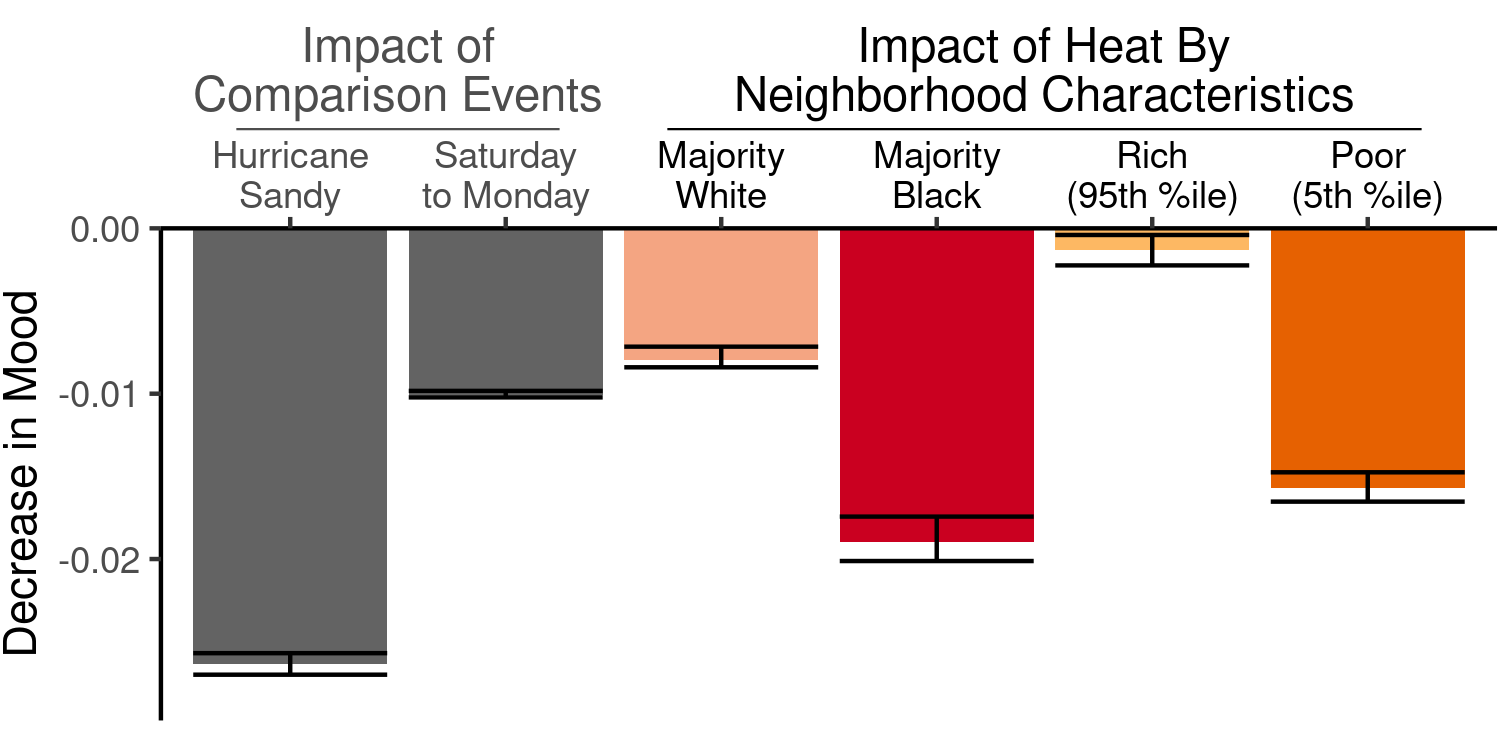
\includegraphics[width=\linewidth]{../res/comparison_plot.png}
  \caption{Decline in sentiment during a heat wave across several different neighborhoods, compared with other impacts on sentiment, such as major hurricanes, as well as the weekly variation in sentiment from the peak on Saturday to the low on Monday.}
  \label{fig:compare}
\end{figure}

We found that the impacts of heatwaves on sentiment in rich and majority white neighborhoods were less than the average weekly change in sentiment from Saturday to Monday, but the effects of heat waves on majority black or poor neighborhoods were much greater than the average weekly change in sentiment.  Additionally, the impacts of heat waves more vulnerable neighborhoods were near to the impacts of Hurricane Sandy.

{\color{red} What other disasters/comparison events should we look at?}

\subsection{Effects by Combined Statistical Area}

To further explore our findings, we examined inequalities in the impacts of higher temperatures on sentiment by Combined Statistical Areas (CSAs) and Metropolitan Statistical Areas (MSAs) with over 1 million people (hereafter: cities).  We examined the change in size of the gap in sentiment scores between both poor and rich neighborhoods, as well as black and non-black neighborhoods, as temperatures change from optimum temperatures of 5\textdegree C WBGT (12\textdegree C/54\textdegree F) to 30\textdegree C WBGT (42\textdegree C/108\textdegree F).

We found increasing inequalities in sentiment across income groups for 68.8\% of cities, with 35.6\% of these having a statistically significant effect (15 cities).  Cities with a significantly unequal effect were found in the south, midwest, northeast, northwest, and southwest, although they were most common in the mid-atlantic region.  Additionally, many cities in the southwest had an inverted effect, where higher temperatures actually narrowed the gap in sentiment between rich and poor neighborhoods, including Denver and Oklahoma City, which had a statistically significant inverted effect.

Because we found a much stronger effect for the effects of temperature on sentiment in majority black neighborhoods, we also examined increases in sentiment gaps between black and non-black neighborhoods in cities with a black population greater than 5\% of the total population.  We found increasing inequalities in sentiment for more black neighrborhoods in 64.7\% of cities, with a significant effect in 21.2\% of those (7 cities).  Additionally, three sunbelt cities had a significant inverted effect.  The patterns of inequalities in the impacts of heat on sentiment by race were similar to inequalities by income: cities with large and significant inequalities were found the mid-atlantic and midwest, as well as central florida.

\begin{figure}[H]
\centering
\begin{subfigure}{0.75\textwidth}
  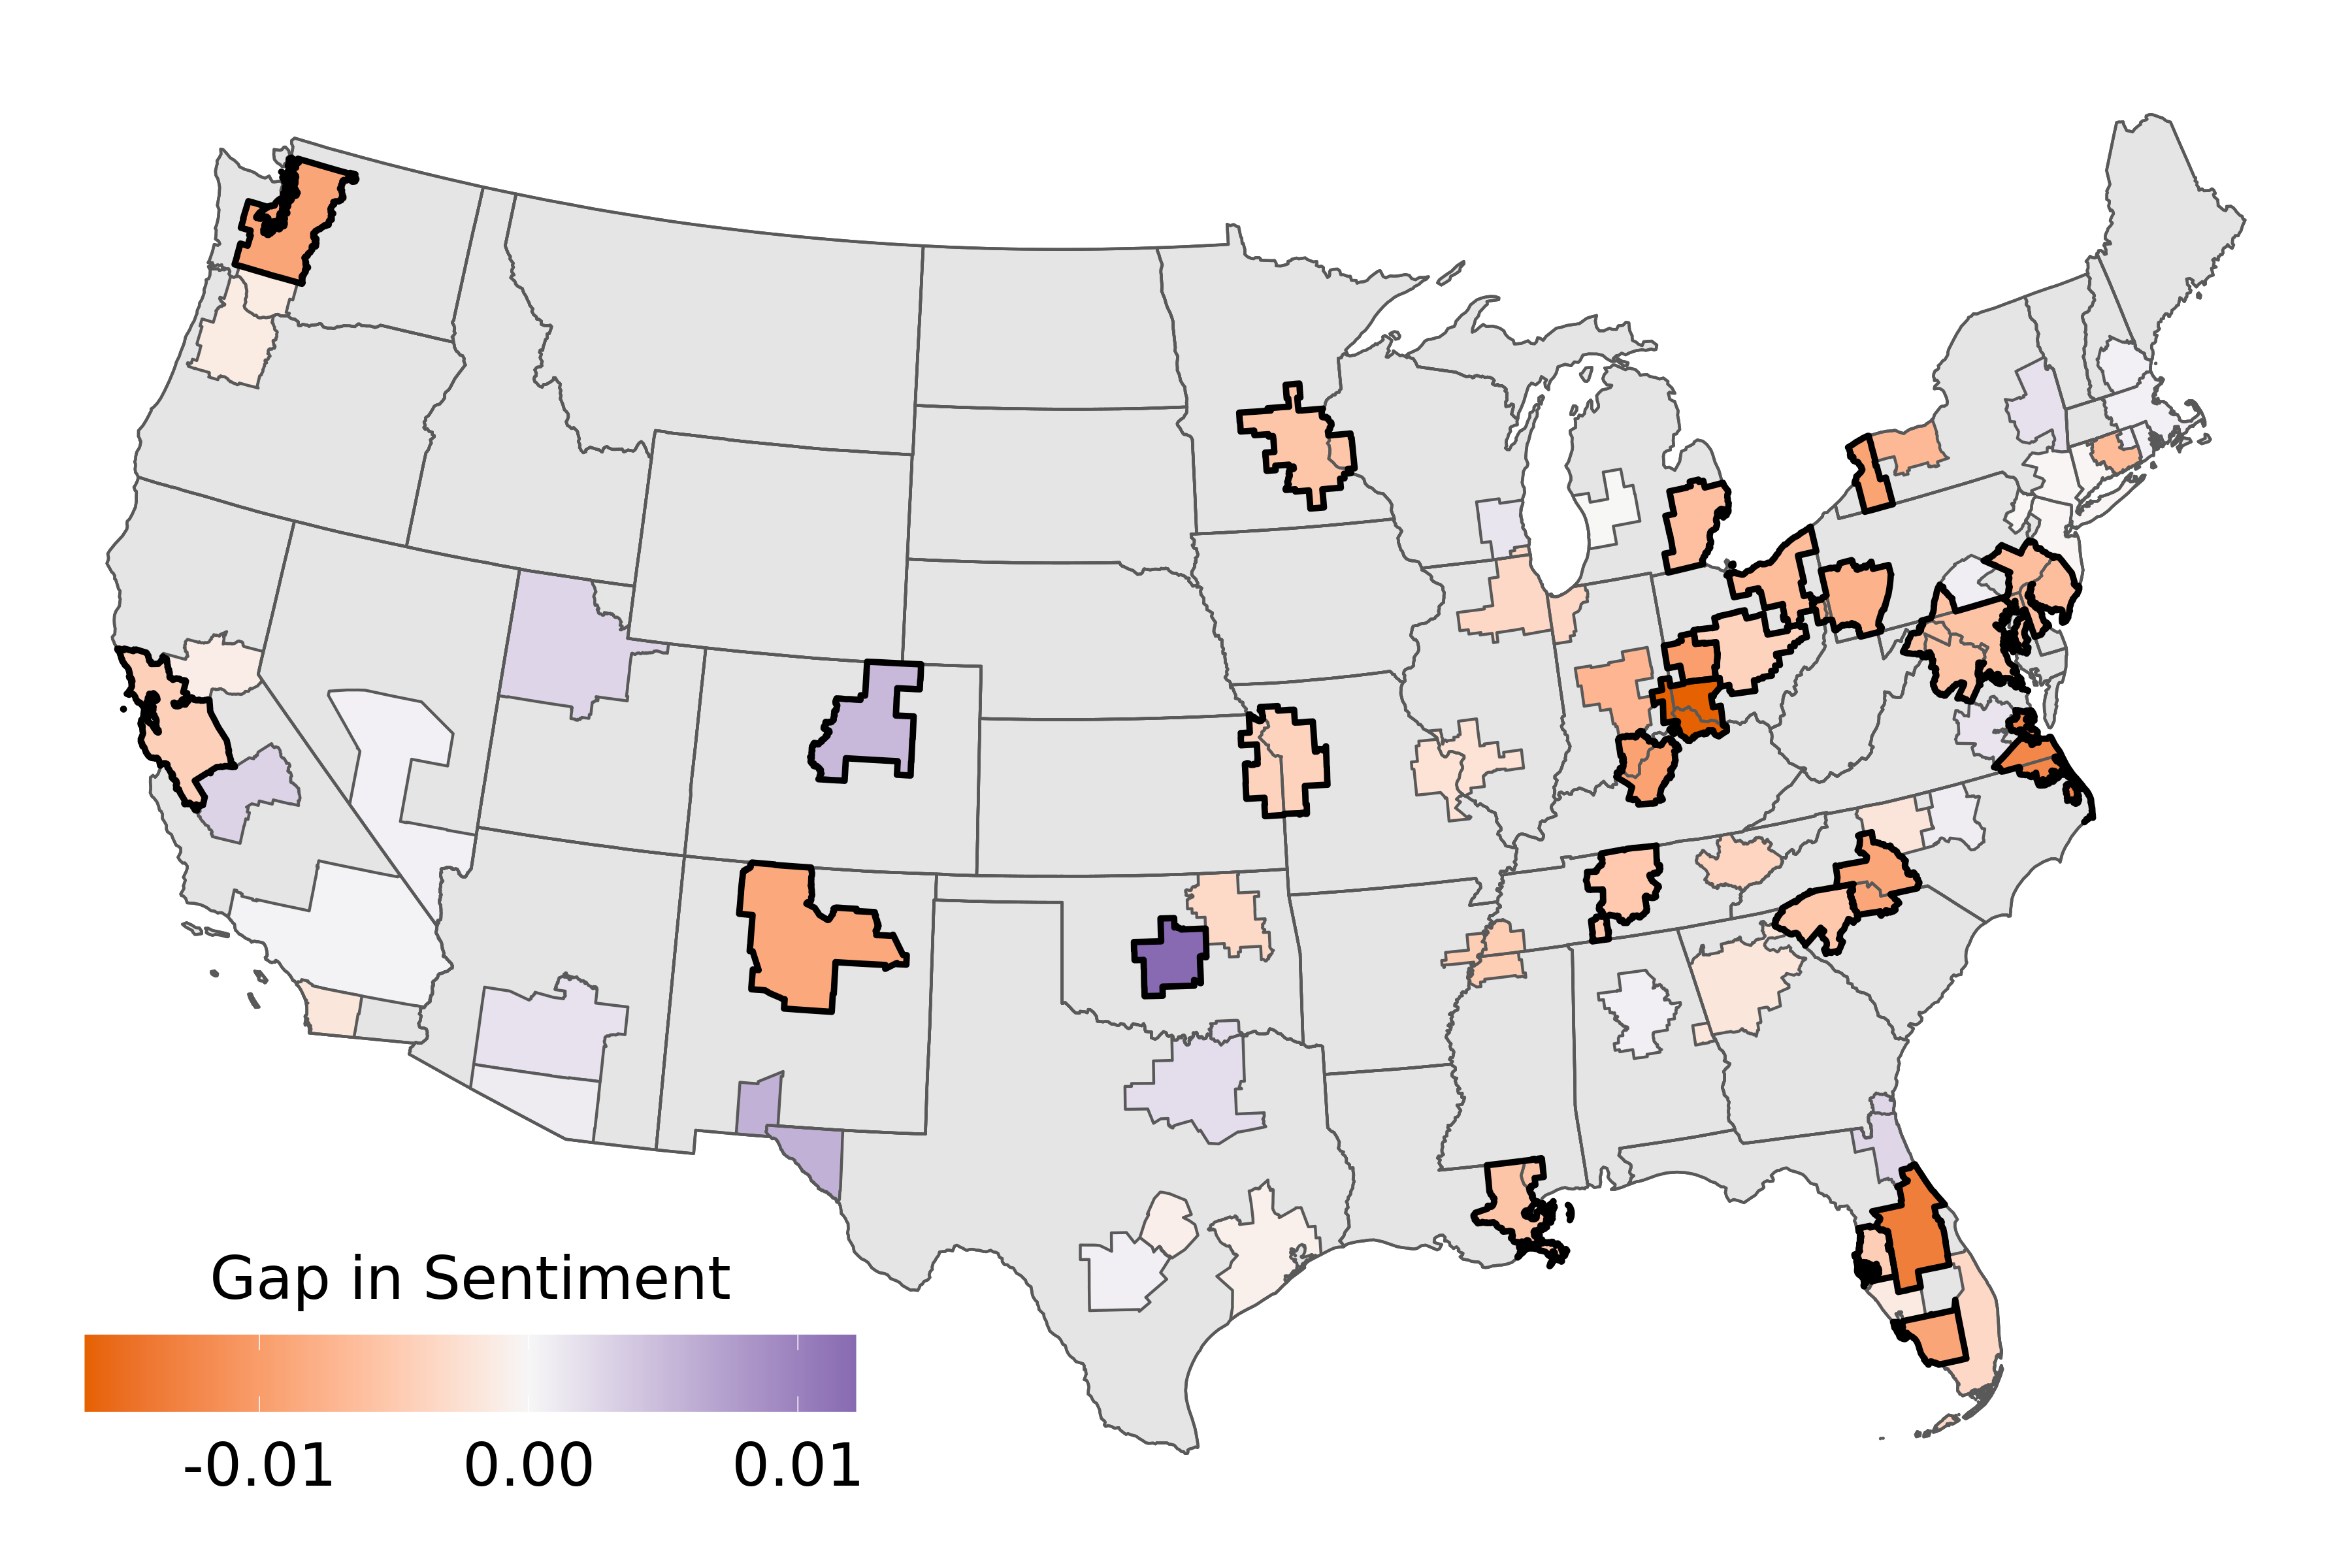
\includegraphics[width=\linewidth]{../res/map_wbgt_income.png}
  \caption{}
  \label{fig:map1}
\end{subfigure}
\begin{subfigure}{0.75\textwidth}
  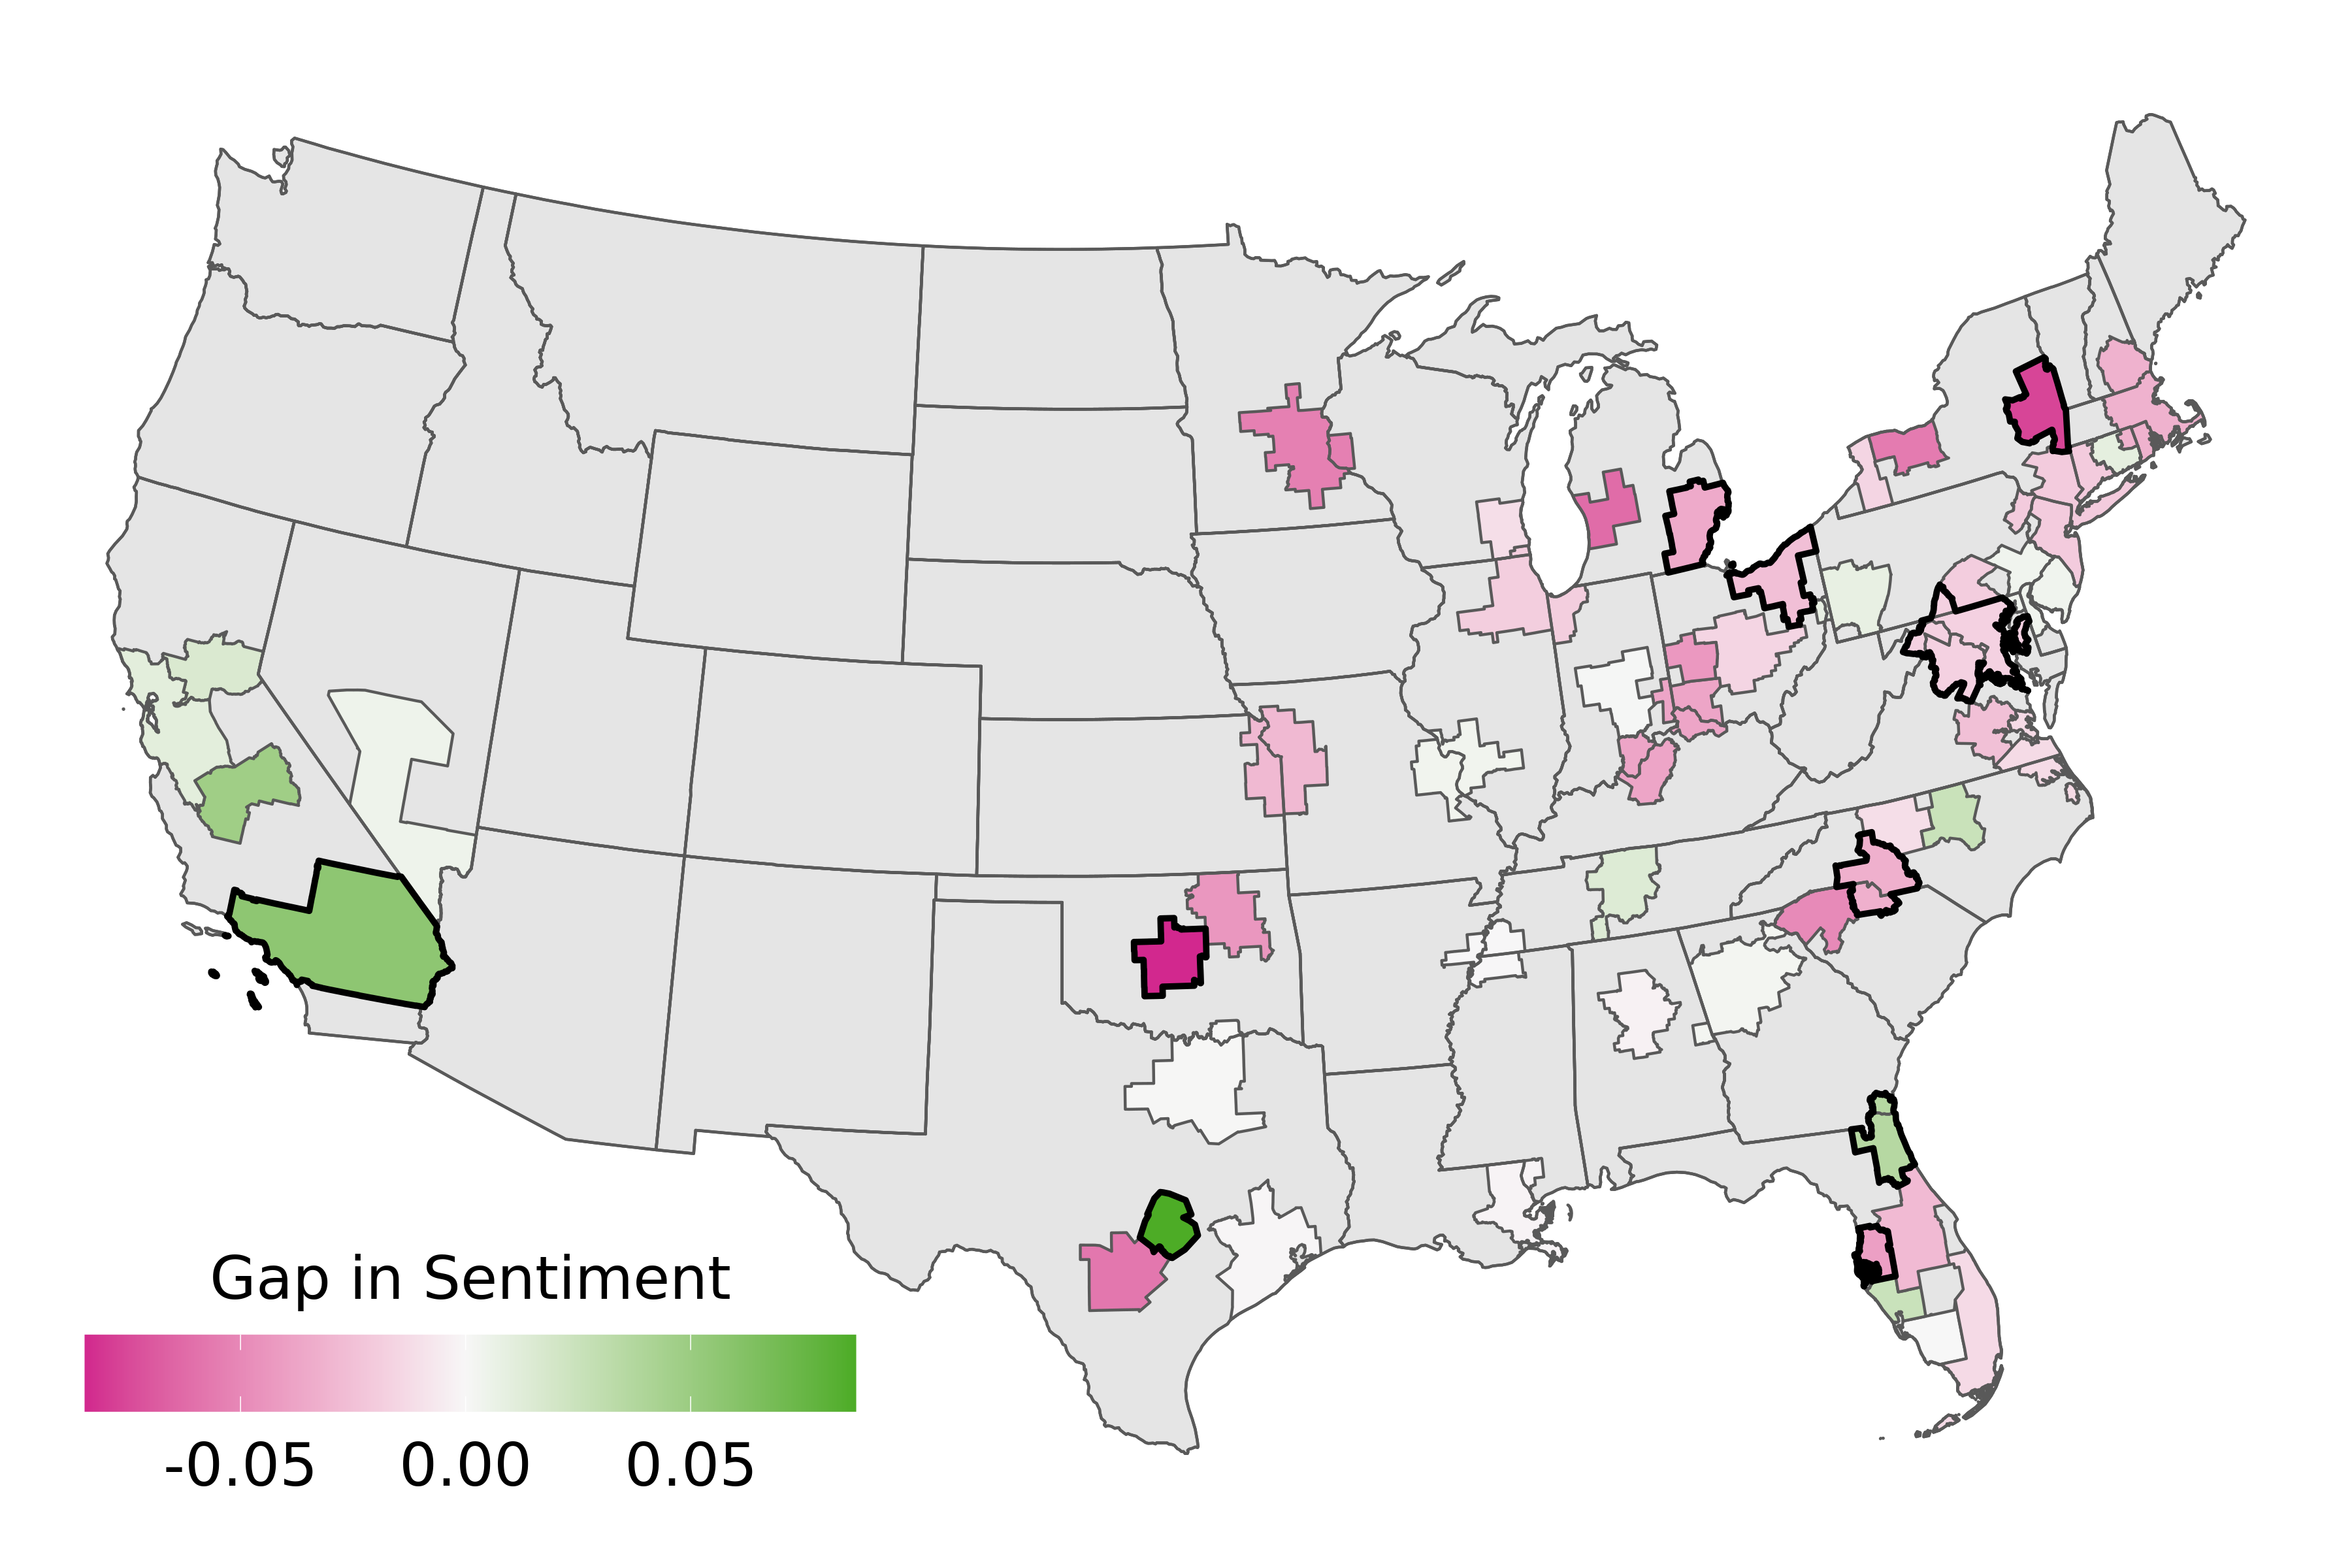
\includegraphics[width=\linewidth]{../res/map_wbgt_black.png}
  \caption{}
  \label{fig:map2}
\end{subfigure}
\caption{Inequalities in impacts of temperature on sentiment by CSAs and MSAs with over 1 million people.  The value shown is the predicted change in the size of the gap in vader score as temperatures increase from 5WBGT to 30WBGT between the 5th and 95 percentile for income (a) and the 95th and 5th percentile for percent black (b).  CSAs with a statistically significant effect ($p < 0.05$) are outlined in black.  For racial inequalities (b), only MSAs and CSAs where black people make up >5\% of the population are included.}
\label{fig:test}
\end{figure}

\subsection{Effects by Time of Day}

In addition to providing data with high spatial resolution, twitter data also comes with very high temporal resolution as each tweet is time-stamped.  Thus, we were able to examine the impact of heat on sentiment for each hour of the day (See Fig. \ref{fig:ts-wbgt}).  We found that heat decreased expressed sentiment at nearly all hours of the day, and that heat had the largest effect on sentiment early in the morning, between 4am and 6am.  Heat had the weakest effects on sentiment at midday, and at 3am.

\begin{figure}[H]
  \centering
  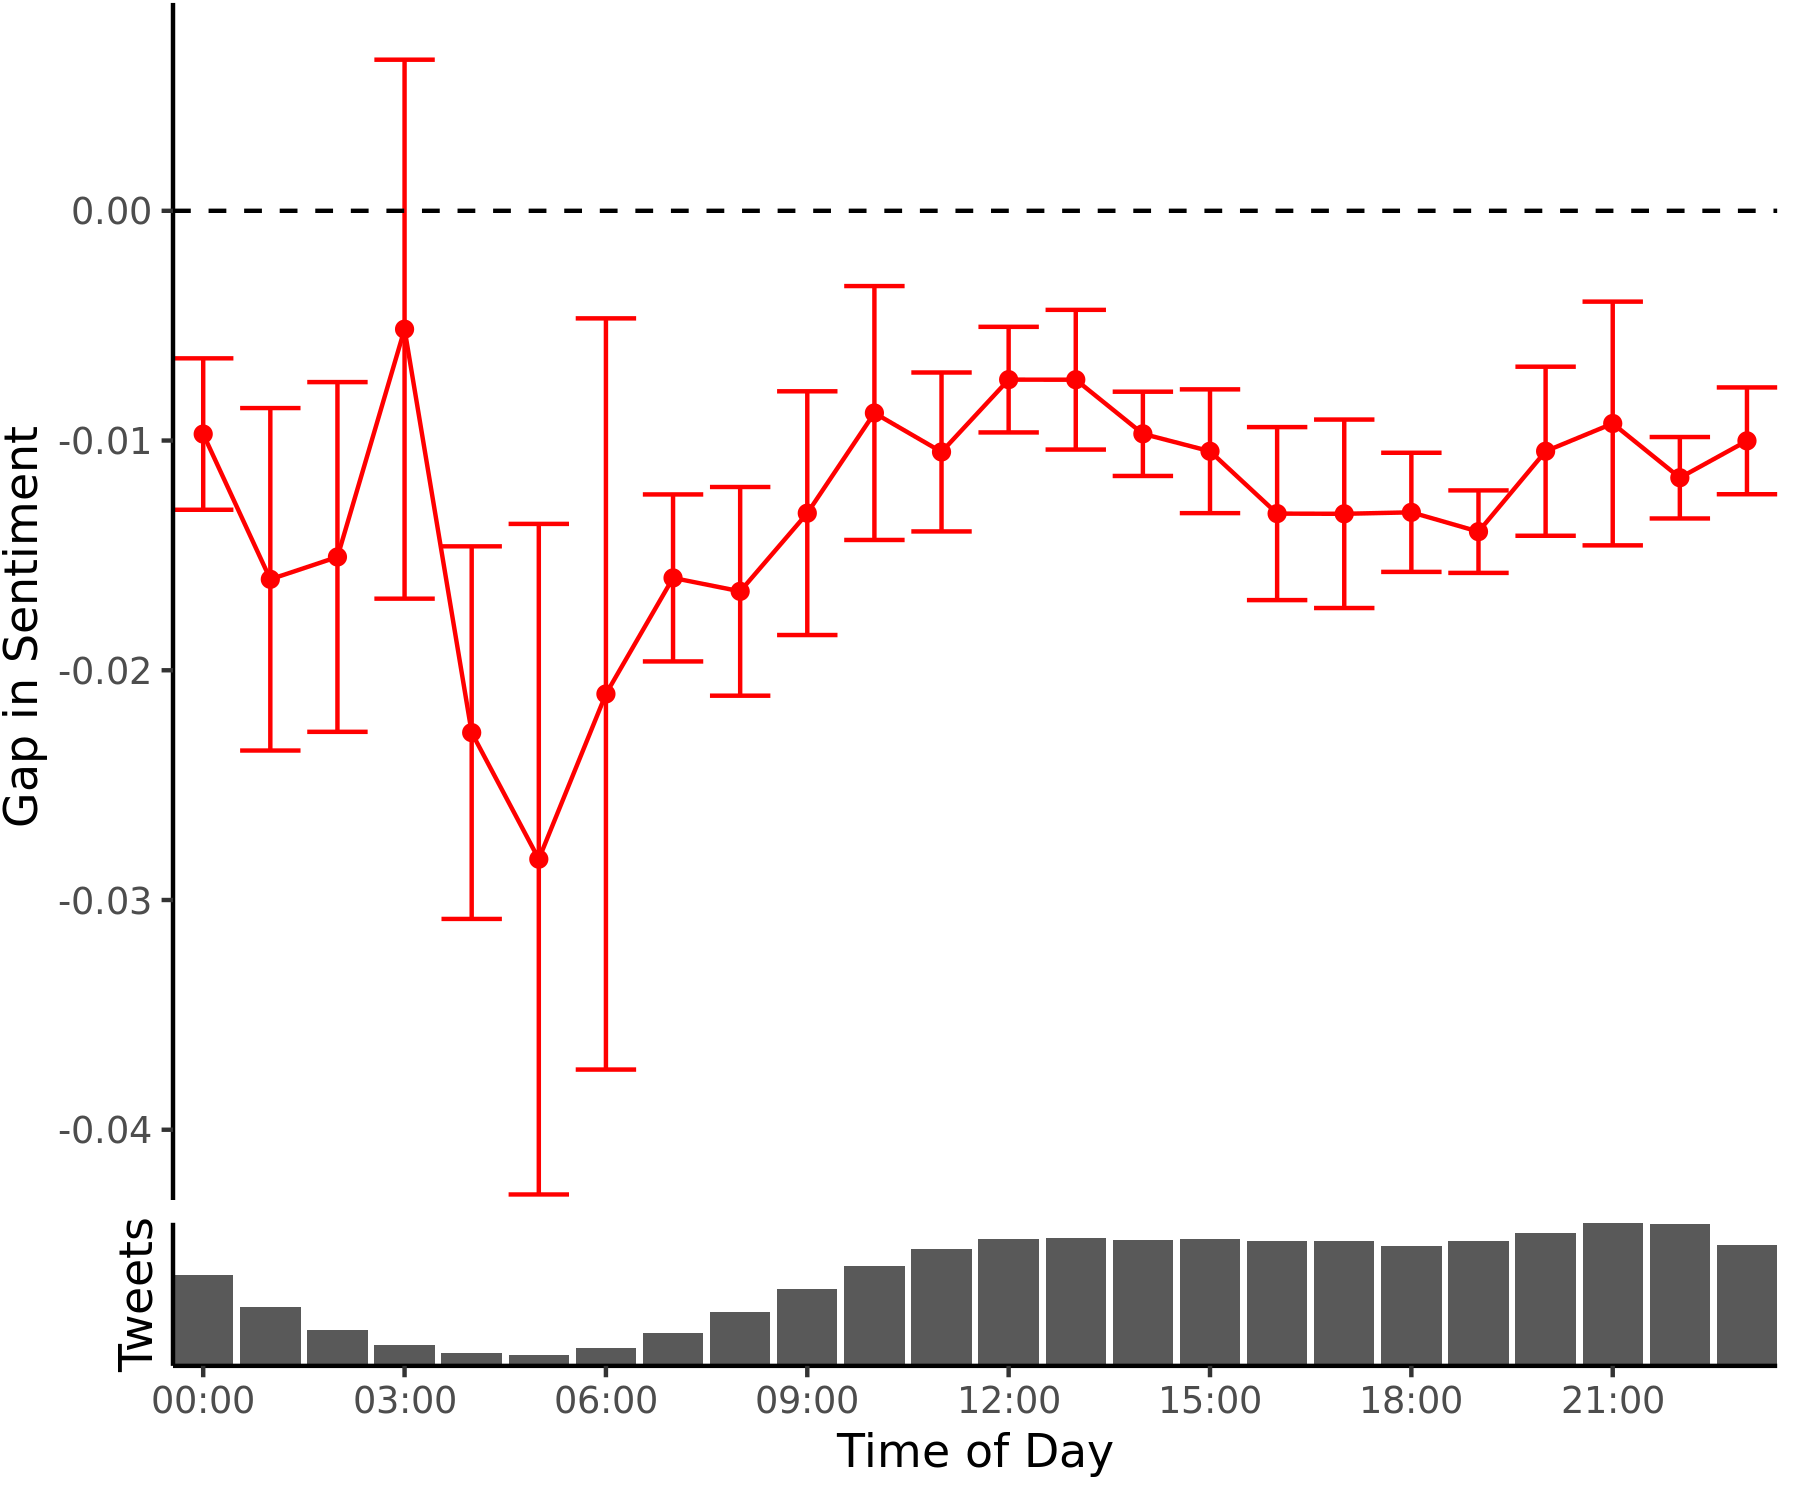
\includegraphics[width=0.5\linewidth]{../res/ts.png}
  \caption{Effects of rising temperatures on sentiment by hour of the day, with a 95\% confidence interval.  The value shown is the predicted change in vader score for a 25-degree increase in temperatures.}
  \label{fig:ts-wbgt}
\end{figure}

\section{Discussion}
% Benefits of twitter data/overview of findings
We found that twitter data offers significant advantages for observing environmental effects on human well-being due to its very fine spatio-temporal resolution.  We were able to pair each tweet with the local temperature at the time of the tweet, and found a clear association between heat and worsened sentiment.   Moreover, we were able to show clear heterogeneities in vulnerability by neighborhood characteristics, overturning previous findings that found no heterogeneities at the county level \cite{Burke2018Aug, Mullins2019Dec}.

% Sentiment is a fuzzy indicator but we have BIG DATA
However, one limitation of data from twitter is that a tweet is not a precise measurement of a discrete mental health outcome and only provides a rough indicator a user's mental state based on the vocabulary in the tweet.  Moreover, while sentiment analysis algorithms have gotten increasingly sophisticated at estimating the mood in a body of text, a users expressed sentiment in a tweet is highly variable and is mostly affected by factors like current events and the user's personal life, with local weather conditions having only a small impact.  We overcome this limitation by using an extremely large dataset of nearly 250 million tweets, allowing us to control for a wide variety of spatial and temporal effects to estimate population-level changes in sentiment in relation to the weather.

% Compare weekly changes in sentiment to weekly changes in suicides
We found that the change from optimum temperature of 5\textdegree C WBGT (12\textdegree C/54\textdegree F) to a heatwave of 25\textdegree C WBGT (36\textdegree C/97\textdegree F) is associated with an overall decrease in the vader sentiment score of 0.01.  This is similar to the degree of change in sentiment over the course of a week from a Monday nadir (0.1268) to a Saturday peak (0.1372), a change in sentiment associated with a suicides increase of 23\% over the course of the study period \cite{CDC2021}.  Thus, while research on linkages between sentiment and other mental health outcomes like suicides and hospitalizations is still nascent, there are clear similarities in patters of sentiment and suicides at some time scales.  Moreover, both suicides and sentiment are affected by higher temperatures \cite{baylis_weather_2018, Burke2018Aug}.  Thus, while twitter sentiment is the only mental health indicator available at fine enough spatial and temporal scales to examine neighborhood and hourly effects, these changes in sentiment are representative of real human suffering, and are also very likely indicative of medical outcomes like suicides and hospitalizations, although this analysis cannot speak to those outcomes specifically.

% Comment on interpretation of results
We examined our results relative to an optimal baseline temperature of 5\textdegree C WBGT (12\textdegree C/54\textdegree F), as this was the temperature at which the highest sentiment scores were observed in the aggregated analysis (See Fig. \ref{fig:wbgt}).  However, after examining heterogeneities by neighborhood race and income, we find different optima for different racial groups and income levels.  For example, the optimum temperature for poor neighborhoods is 0\textdegree C WBGT (6\textdegree C/43\textdegree F) while the optimum temperature for rich neighborhoods is 20\textdegree C WBGT (29\textdegree C/84\textdegree F).  These different varying optima show that even mild heat can affect human well-being, and the only reason that sentiment peaks as high as 20\textdegree C WBGT (29\textdegree C/84\textdegree F) in rich neighborhoods is because the rich are more likely to have air conditioning in their homes, transportation, and work spaces, as well as much greater choice in when they are outside and in the activities they perform outside.

% Comment on Race, why no effect on hispanics?
We found that majority black neighborhoods are much more affected by heat than neighborhoods with a majority of any other race.  This is surprising, given that Hispanics can be marginalized in both income and housing.  This finding may be because the racial category of Hispanic is more broad and encompasses many more groups with more diverse histories and income levels than black Americans.  Additionally, there are many other marginalized groups in America, particularly indigenous people, that we did not have sufficient data to examine with respect to heat and mental health.  

% Interpret Spatial Analysis
In our spatial analysis, we found that most cities exhibited both racial and income inequalities in the vulnerability of mental health to heat, with noticeable regional patterns in the strength of the effect.  Generally, the mid-west and mid-atlantic had the strongest inequalities, and the south-west had the weakest inequalities and an occasional inverted effect.  Because we used Wet Bulb Globe Temperature, our metric accounts for how differences in humidity and wind speed affect the human body's ability to cool itself through perspiration.  Thus, this regional differences in vulnerability are likely more due to cultural or infrastructural differences than to different environmental conditions.

% Interpret Time Series Analysis
Recent research has suggested that the impacts of heat on sleep quality may play a large role in the observed mental health effects of heat \cite{Obradovich2017May, Mullins2019Dec}, and our temporal analysis was able to examine this hypothesis.  While our estimates were more uncertain at night due to a lower volume of tweets, we found much stronger effects of heat on expressed sentiment in the early morning, adding weight to the sleep quality pathway linking heat and mental health that other authors have found.  This suggests that efforts to improve mental health during heat waves may have the largest impact by focusing on providing electricity and air conditioning at night.

% Caveats
While these findings are robust to different model specifications and sentiment metrics, there are some caveats.  For one, we were only able to locate the tweets within the census block where the tweet was sent - we did not to infer where the person sending the tweets typically lived or where they had been.  Many low-income and black people commute during the day to work in the service sector in higher-income areas, so these results may in fact under-estimate the impacts of higher temperatures on mental health for poor and minority individuals.  Moreover, the income level of a census block may be only weakly correlated with the wealth of the people who are typically found that census block.  For example, some public spaces are estimated to have very low income levels even though people from a variety of income levels may occupy those spaces throughout the day.  Additionally, neighborhoods of young college students are also typically estimated to have low income levels, even through college students are wealthier than the average American.  Again, these issues mean we are likely under-estimating the true effect of heat on mental health.  A final issue with using twitter data is that, while twitter is used by more than one in five Americans, twitter users may not be representative of the general population, as they are typically younger, wealthier, and more educated \cite{Pew2020Sep}.  Nevertheless, we found a large volume of tweets across all neighborhood types.

% NCC doesnt have a "conclusion" section, but this is intended as an overall summary paragraph
While climate change will have widespread and severe impacts on human well-being, these impacts are will be highly unevenly distributed.  People with more money, access to aid and infrastructure, and who belong to ethnic groups in power are less affected by climate shocks and natural disasters \cite{bullard2012wrong}.  While the physical health impacts of these shocks are more visible and easy to measure, there is no reason to believe that the mental health impacts of climate change will not also be highly unevenly distributed.  Thus, there are strong theoretical priors behind the hypothesis that low-income and marginalized people are more vulnerable to the mental health impacts of higher temperatures, even though previous work at coarse spatial scales has not found such an effect.  By using fine-scale twitter data, we showed that there are indeed stark difference in the mental health impacts of heat among neighborhoods in America.

\section{Methods}

% A proposed list of tables and figures:
% Figures of income blocks and temperature extremes.
% Table 1. Variable descriptions for what's included in our models.
% Table 2. Descriptive statistics for datasets/variables we include.
% Table 3. Model results with variables included in the models coefficients, SEs, p-values, sample size.

\subsection{Tweets \& Sentiment}
We used data from 243 million geo-located English-language tweets from the lower 48 states from the years 2009 to 2019.  The Twitter data consists of publicly posted messages, or Tweets, that are short status messages users post to the platform.  We only considered users’ original content, thus did not include retweets in our analysis.  Additionally, we excluded all tweets that contained weather-related terms, to ensure that the sentiment expressed in the tweets was reflective of a user's mental state, and not a commentary on the weather.

We assessed the sentiment expressed in the tweets using the VADER (Valence Aware Dictionary for sEntiment Reasoning) sentiment corpus \cite{gilbert_vader_2014}. VADER is a lexicon and rule-based sentiment analysis tool that is specifically attuned to sentiments expressed in social media because of several features, as:

\begin{itemize}
  \item Incorporating lexical features common to informal media, such as slang (``sux"), and acronyms (``lol").
  \item Negations (``\textit{not} good", ``\textit{wasn't} bad")
  \item Punctuation (``Good!!!")
  \item Word shape, such as capitalization (``The move was AMAZING")
  \item Emoticons and emojis (``:-)", ``\emojismile")
  \item Degree modifiers (``very excellent" or ``kind of crappy")
\end{itemize} 

The VADER method yields a value for the mood of a tweet, with a score of 0 for neurtral tweets, a score $> 0$ for positive-mood tweets and a score $< 0$ for negative-mood tweets.  In addition to the vader method used in the body of this paper, we also conduct our analysis using the Hedonometer and AFINN sentiment analysis methods, with similar results (See Appendix).

Some papers we might cite in this section (only for multilingual work): Vilares et al. 2017 , Lo et al. 2017, Dashtipour et al. 2016.

Discuss issues with text data (gtp) - that it doesn’t capture emoticons, code switching (e.g., [good job! \#fail]), etc.

Issues with what people say on social media being attenuated or mismatched from actual emotional state


\subsection{Weather}
We used data on local weather conditions from the North American Land Data Assimilation System (NLDAS), a gridded product developed by several collaborative institutions, including NOAA, NASA, Princeton University, and the University of Washington.  This dataset is available at an hourly temporal resolution, and at 1/8th decimal degree spatial resolution, and integrates a large quantity of observation-based and modeled data  \cite{xia_continental-scale_2012}.  For the exact hour and location of each tweet, we extracted temperature, specific humidity, air pressure, total precipitation, shortwave radiation, and wind speed.  

Because metrics of apparent temperature that take into account humidity and other factors can better account for the impacts of heat stress on human health and wellbeing, we calculate the Wet Bulb Globe Temperature (WBGT) at the time and location of each tweet.  WBGT is the temperature that a wet globe thermometer would read in direct sunlight, and gives a reading lower than a dry bulb temperature would show due to evaporative cooling, and can be estimated given normal temperature, relative humidity, solar radiation, and wind speed.  Because evaporative cooling is how humans cool themselves through perspiration, this temperature better indicates the heat stress that people are experiencing.  Metrics like WBGT that account for the effects of humidity and other factors on heat stress have been associated with diminished economic output \cite{rao2020projections}, increased crime \cite{hu2017impact}, increased mortality \cite{chien2016spatiotemporal, armstrong2019role}, and worsened mental health outcomes \cite{vida2012relationship, ding2016importance}.

Using temperature, specific humidity, and pressure, we derived relative humidity using methods described by  \cite{bolton_computation_1980}.  We then calculated the WBGT using the formula described by \cite{heo2019comparison}.

\subsection{Socio-Econoimc Data}
We used data from the American Communit   Survey administered by the US Census to income levels and the racial composition of neighborhoods where tweets were located.  Data was at the level of the census block group, the smallest unit for which the census releases public data.

ACS data is released to cover five-year periods.  We therefore matched each tweet with census block group data from the year at the middle year of each survey's five-year range.  For example, tweets from 2014 were matched to data from the 2012-2016 ACS.  Because the most recent available data was from 2014-2018, all tweets from year years greater than 2016 were matched to this dataset.  Data was downloaded from the IPUMS NHGIS service provided by the University of Minnesota.

Mean annual income per capita is provided by the ACS, and we standardized this variable so that the values for each year were in 2019 dollars.  For racial categories, we combined the various categories provided by the ACS into four racial groups: non-Hispanic white, non-Hispanic black, Hispanic of any race, and an "other" category for non-Hispanic people who were neither black nor white, such as Asian, Native American, or mixed-race people.


\subsection{Modeling}
We assessed how expressed sentiment is affect by three weather variables: wet bulb globe temperature, precipitation, and sunshine.  Moreover, we modeled how neighborhood income affects the relationship between these weather variables and sentiment.

Our model takes the following form:
\begin{equation}
    y = \beta_0 + f_t(t) + f_{mt}(m t) + \beta_p p + \beta_{mp} m s + \beta_s s + \beta_{ms} m s + \Phi + \epsilon
\end{equation}

Where $y$ is the sentiment of a tweet, $t$ is the wet bulb globe temperature at the hour of the tweet, $p$ is a binary variable indicating whether it rained at the hour of the tweet, $s$ is the income shortwave radiation, or sunshine, in $W/m^2$, at the hour of the tweet, and $m$ is the log-transformed average income in the census block where the tweet originated.  We estimate the 


STANDARD ERRORS


\section{Acknowledgements}
This work was supported by the National Socio-Environmental Synthesis Center (SESYNC) under funding received from the National Science Foundation DBI-1639145.  Additionally, cloud resources for this project were provided for the Microsoft Azure cloud by Microsoft's AI for Earth program, grant number .

This data came from Twitter via the University of Vermont’s (UVM) agreement with Twitter to access its streaming API - colloquially referred to as the Decahose.  The UVM special agreement with Twitter allows for access to this data for research and analysis purposes and we have complied with all the terms of service for Twitter and UVM. 
\printbibliography

\end{document}
